\chapter{Simulated Annealing Implementation}
\label{ch:sa}

\section{Code structure: Algorithm $\rightarrow$ Feasibility $\rightarrow$ Engine}
The code is organised as a pipeline of three independent layers (Figure~\ref{fig:arch}). The
\emph{algorithm} only sees a box of numbers and a cost; the \emph{feasibility} layer decides whether
a vector describes a mission that may fly; the \emph{engine} simulates feasible missions and
returns $J$. A design that fails a pre-engine check never reaches the (expensive) engine and
receives the penalised cost~(\ref{eq:penalty}) directly. Because the algorithm only relies on a
small \texttt{Problem} interface (bounds, variable kinds, \texttt{repair}, \texttt{evaluate}),
the same \ac{SA} code also runs on standard benchmark functions (validation V2), and the
algorithms of later milestones (GA, PSO) plug into the same pipeline through a registry.

\begin{figure}[htbp]
\centering
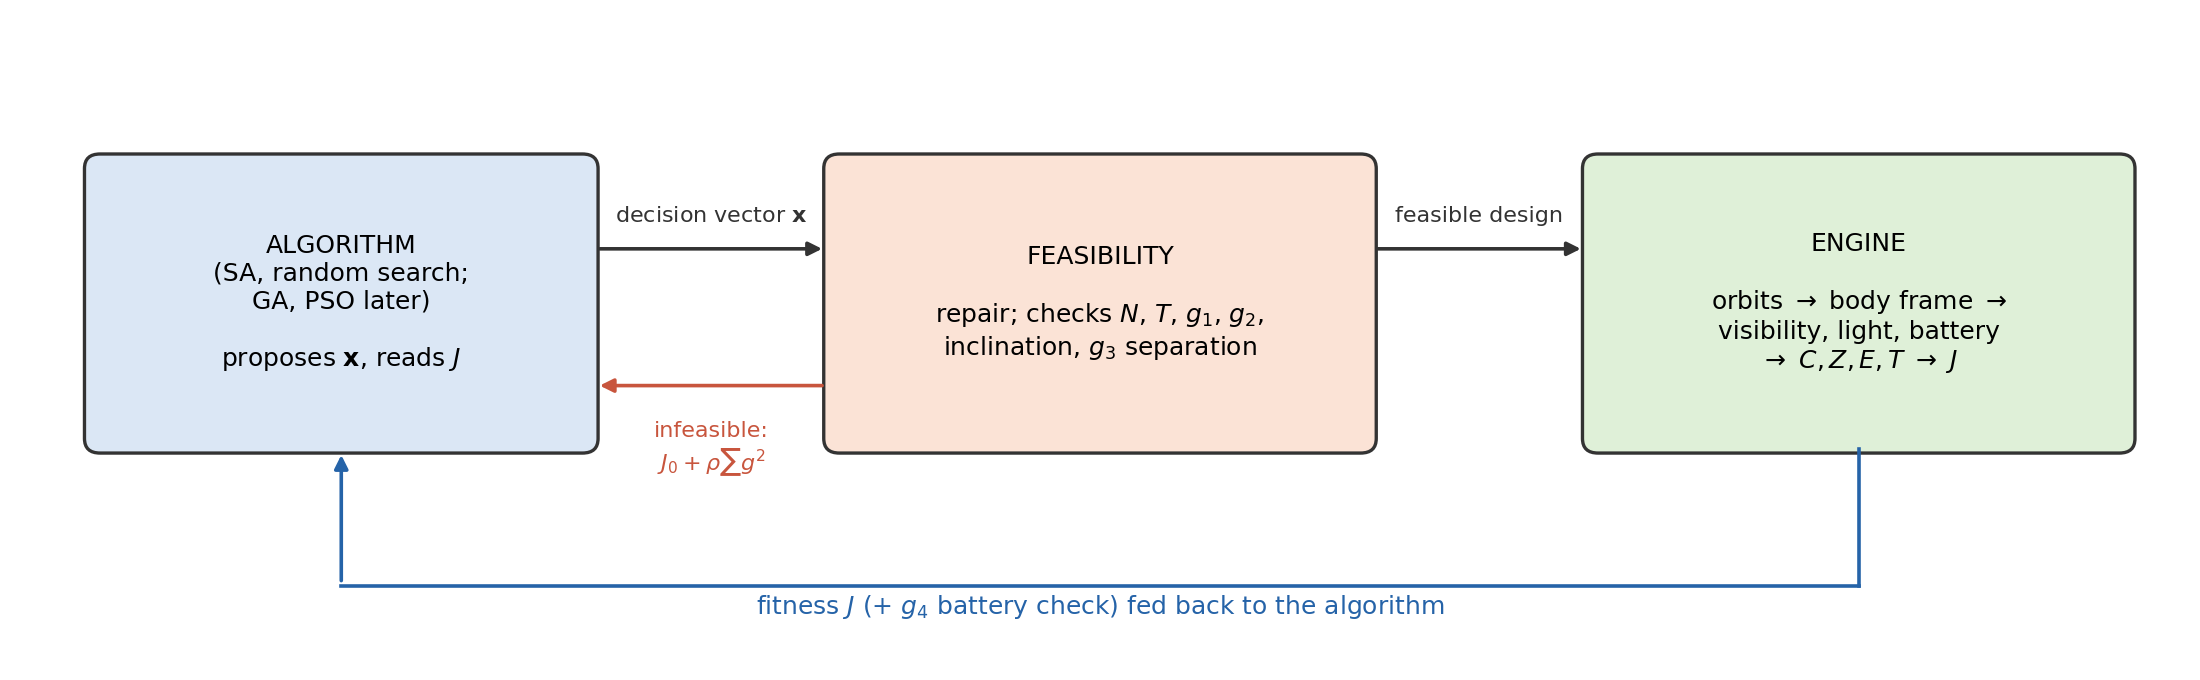
\includegraphics[width=\textwidth]{Figures/architecture.png}
\caption{The optimisation pipeline. The algorithm proposes a decision vector; the feasibility layer
rejects (with a penalty) or passes it; the engine simulates the mission and returns the fitness,
which is fed back to the algorithm.}
\label{fig:arch}
\end{figure}

\begin{table}[htbp]
\centering
\caption{Main code modules (package \texttt{spacecov})}
\label{tab:modules}
\footnotesize
\begin{tabularx}{\textwidth}{@{}p{5.6cm}X@{}}
\toprule
Module & Content \\
\midrule
\texttt{config.py} & all mission, constraint and cost parameters; body presets (Eros, Kleopatra) \\
\texttt{design.py} & decision vector layout, bounds, variable kinds, encode/decode (Eq.~\ref{eq:x}) \\
\texttt{feasibility.py} & constraints of Table~\ref{tab:constraints}, the \texttt{repair} operator \\
\texttt{physics.py} & stages 1--4 of Chapter~\ref{ch:orbital} for one spacecraft \\
\texttt{engine.py} & track cache, fleet simulation, objectives and $J$ (Eq.~\ref{eq:J}) \\
\texttt{pipeline.py} & Algorithm $\rightarrow$ Feasibility $\rightarrow$ Engine; the \texttt{Problem} the algorithms see \\
\texttt{algorithms/sa.py} & Simulated Annealing (this chapter) \\
\texttt{algorithms/ga.py} & Genetic Algorithm (Chapter~\ref{ch:ga}) \\
\texttt{algorithms/random\_search.py} & random search with the same budget (baseline of validation V4) \\
\texttt{algorithms/benchmarks.py} & sphere, Rastrigin and Ackley test functions (validation V2) \\
\texttt{experiments/validate.py} & every case study and validation run of Chapters~\ref{ch:cases}--\ref{ch:results} \\
\texttt{viz/} & interactive 3D viewer and live optimiser display \\
\bottomrule
\end{tabularx}
\end{table}

The \ac{SA} loop is written from scratch with NumPy only; no optimisation toolbox or package is
used anywhere in the algorithm.

\section{The algorithm}
\ac{SA}~\cite{kirkpatrick1983} keeps one current design and repeatedly proposes a small change.
A better design is always accepted; a worse one is accepted with the Metropolis
probability~\cite{metropolis1953} $\exp(-\Delta J/\Theta)$, which is high while the temperature
$\Theta$ is high and vanishes as it cools. Early on the search can therefore leave regions that
are only locally good; at the end it fine-tunes the best region. (The temperature is written
$\Theta$ here to avoid confusion with the mission duration $T$.) Algorithm~\ref{alg:sa} gives the
implementation and Figure~\ref{fig:flow} the corresponding flowchart.

\begin{algorithm}[htbp]
\caption{Simulated Annealing for the fleet design}
\label{alg:sa}
\begin{algorithmic}[1]
\REQUIRE budget $B$ evaluations, $n_{\mathrm{init}}=20$, $p_0=0.5$, $\sigma_0=0.25$, $\sigma_{\min}=0.01$, $\Theta_{\min}/\Theta_0=10^{-3}$
\STATE \textbf{Warm start:} draw $n_{\mathrm{init}}$ random designs that pass the pre-engine checks, evaluate them, $\mathbf{x}\leftarrow$ the best
\STATE \textbf{Start temperature:} make 20 trial moves from $\mathbf{x}$; $\Theta_0\leftarrow-\operatorname{median}(\Delta J^{+})/\ln p_0$ over the feasible uphill moves
\STATE $L\leftarrow\max(10,\dim\mathbf{x})$; \quad $n_{\mathrm{lev}}\leftarrow\lceil(B-\text{evaluations used})/L\rceil$; \quad $\alpha\leftarrow(\Theta_{\min}/\Theta_0)^{1/(n_{\mathrm{lev}}-1)}$
\STATE $\Theta\leftarrow\Theta_0$; \quad $\mathbf{x}^{*}\leftarrow\mathbf{x}$
\WHILE{the budget is not used}
  \FOR{$L$ moves}
    \STATE $\sigma\leftarrow\max\bigl(\sigma_{\min},\,\sigma_0\sqrt{\Theta/\Theta_0}\bigr)$ \hfill (moves shrink as it cools)
    \STATE $\mathbf{y}\leftarrow\textsc{Repair}(\textsc{Neighbour}(\mathbf{x},\sigma))$
    \STATE $J(\mathbf{y})\leftarrow$ Feasibility $\rightarrow$ Engine; \quad $\Delta J\leftarrow J(\mathbf{y})-J(\mathbf{x})$
    \IF{$\Delta J\le0$ \textbf{or} $\mathrm{rand}()<\exp(-\Delta J/\Theta)$}
      \STATE $\mathbf{x}\leftarrow\mathbf{y}$ \hfill (Metropolis acceptance)
    \ENDIF
    \IF{$\mathbf{y}$ is better than $\mathbf{x}^{*}$ (feasible first, then lower $J$)}
      \STATE $\mathbf{x}^{*}\leftarrow\mathbf{y}$
    \ENDIF
  \ENDFOR
  \STATE $\Theta\leftarrow\alpha\,\Theta$ \hfill (geometric cooling)
\ENDWHILE
\RETURN $\mathbf{x}^{*}$
\end{algorithmic}
\end{algorithm}

\begin{figure}[htbp]
\centering
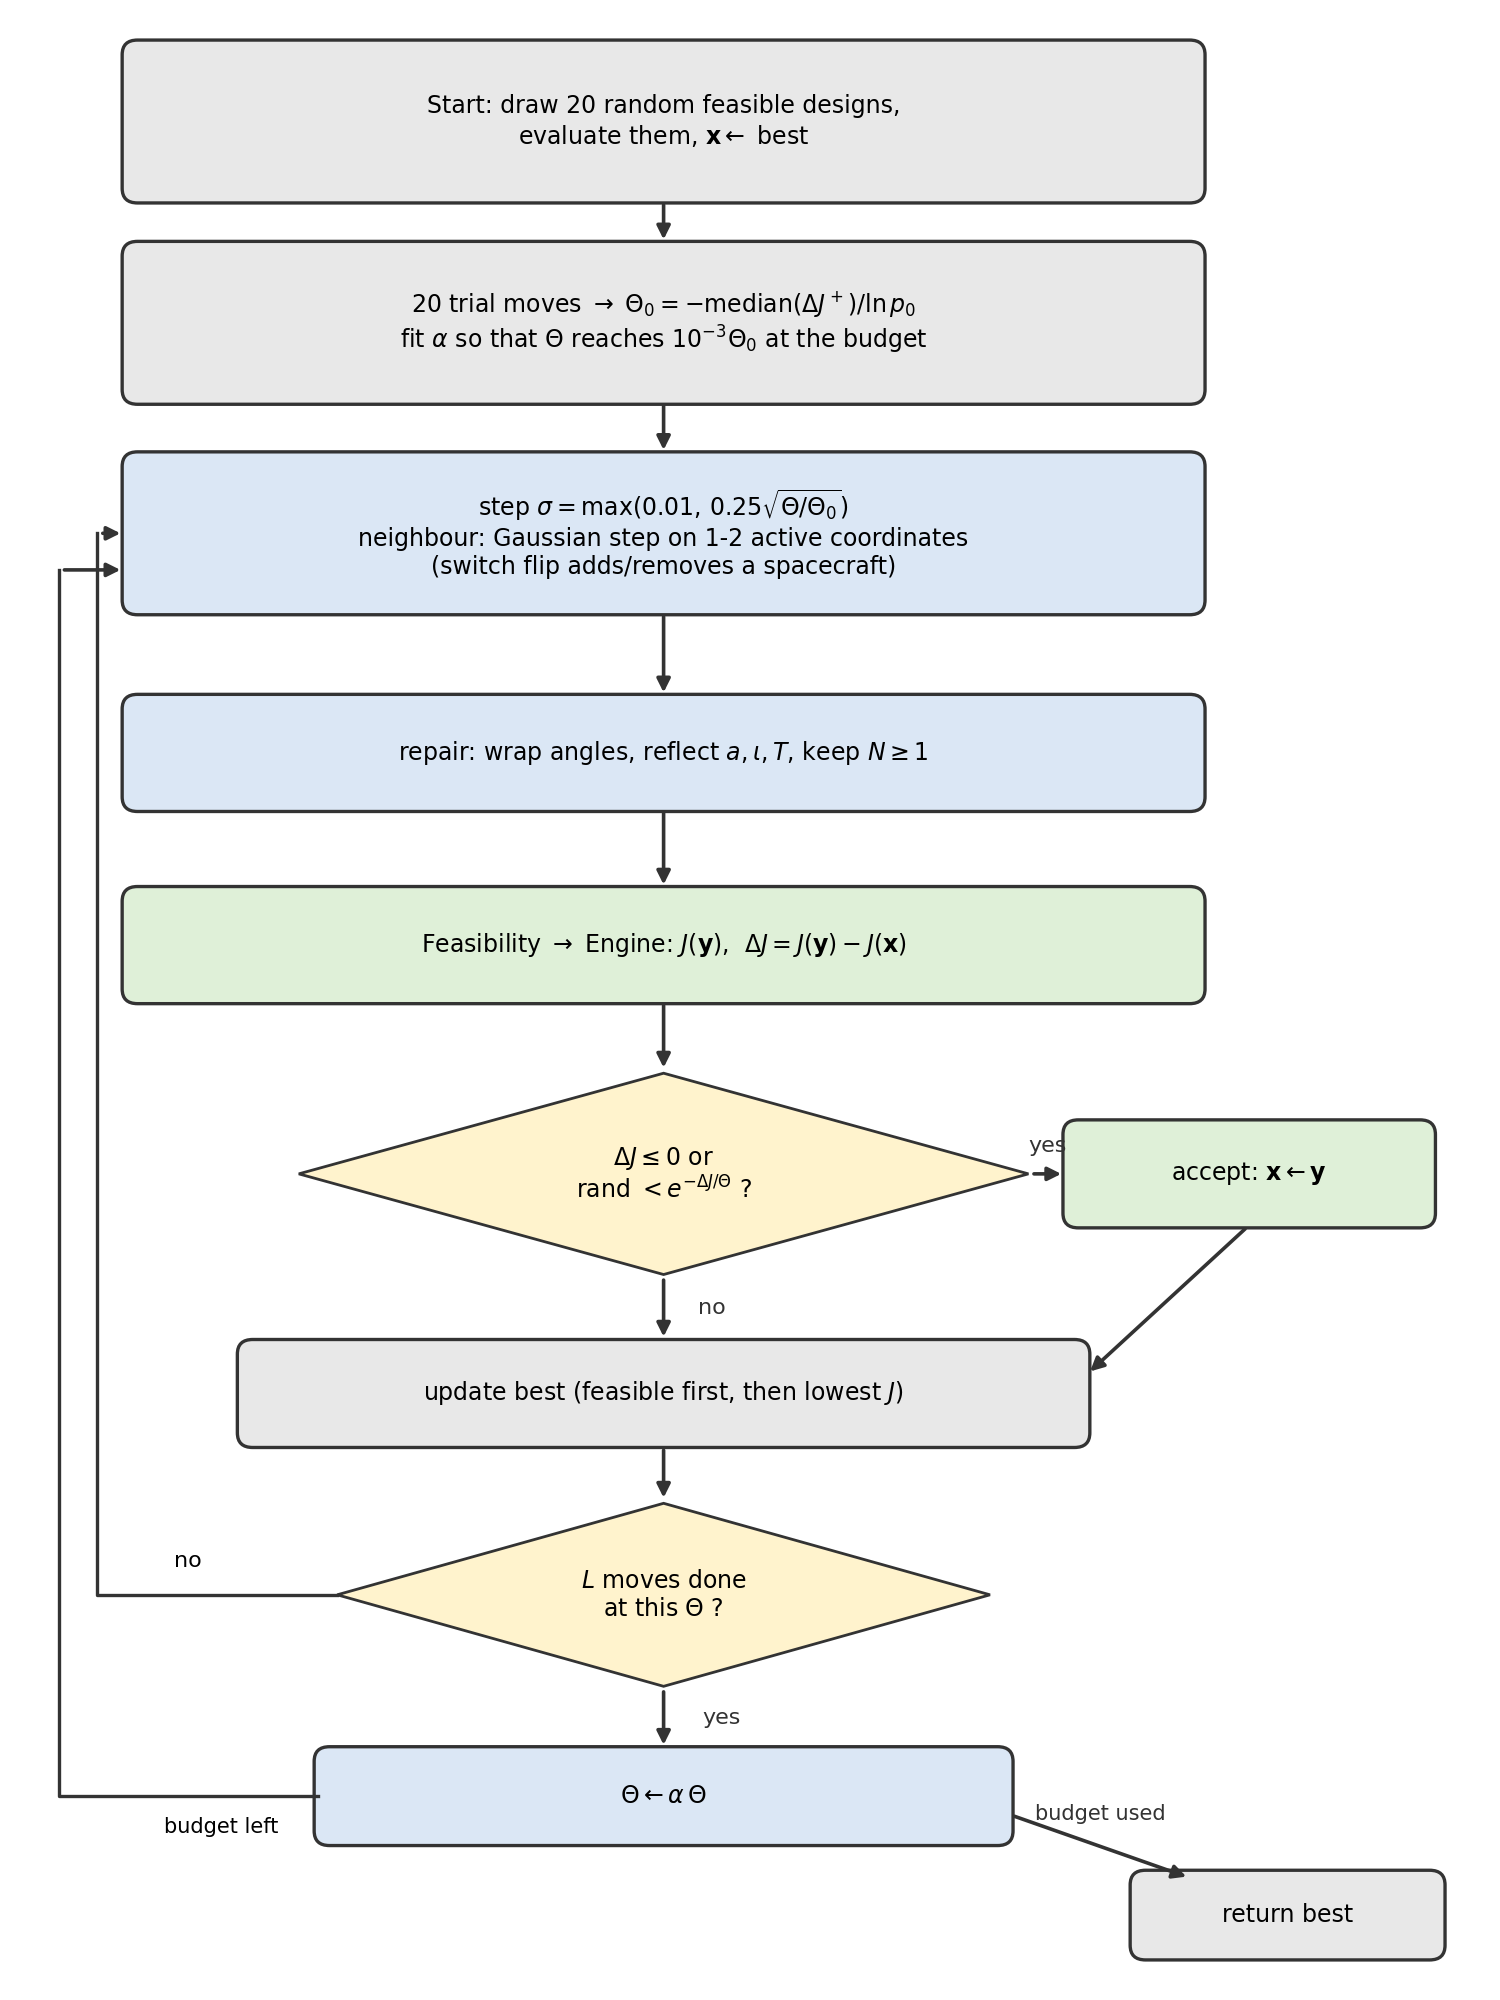
\includegraphics[width=0.78\textwidth]{Figures/sa_flowchart.png}
\caption{Flowchart of the Simulated Annealing implementation.}
\label{fig:flow}
\end{figure}

\section{Problem-specific considerations}
\label{sec:sa-problem}
Table~\ref{tab:saspecific} summarises how the generic algorithm is adapted to the fleet problem.

\textbf{Neighbourhood operator.} A move changes one or two coordinates (chosen with equal
probability), drawn only among the coordinates that currently \emph{matter}: the duration $T$, every
switch $s_i$, and the four orbit variables of the \emph{flying} spacecraft. The orbit numbers of a
switched-off slot are never moved, because changing them would not change the mission and would
waste an evaluation. A real coordinate $j$ receives Gaussian noise
$\mathcal N\bigl(0,(\sigma\,(\mathrm{ub}_j-\mathrm{lb}_j))^2\bigr)$, so the step is a fraction $\sigma$
of the variable's range. A switch is an integer, so it is flipped (the noise is rounded to at least
$\pm1$ and the repair clips it back to 0 or 1): this adds or removes a spacecraft, which is how
\ac{SA} searches the fleet size. One move therefore changes at most one or two spacecraft, and
thanks to the track cache (Chapter~\ref{ch:orbital}) it costs at most two new spacecraft
simulations whatever the fleet size.

\textbf{Repair operator.} After a move the vector is mapped back into the box:
$\Omega_i$ and $M_{0,i}$ wrap around $360^\circ$; $a_i$, $\iota_i$ and $T$ are \emph{reflected} at
their bounds (a step that would leave $[r_{\min},r_{\max}]$ by 3\,km lands 3\,km inside), which keeps
the random walk unbiased near the bounds; switches are rounded to 0 or 1. If a move would switch
off the last spacecraft, the repair switches it back on, so $N\ge1$ always holds. Constraints
$g_1$, $g_2$, the duration range and the inclination range can therefore never be violated by an
\ac{SA} candidate; only separation ($g_3$) and battery ($g_4$) can still fail. A move that the
repair maps back onto the current design, or widens to more than two coordinates, is redrawn, so
every move stays local.

\textbf{Warm start.} The narrow camera only works up to $\ell_{\max}=58.6$\,km (Eros), so a large
part of the box (high orbits, short missions) photographs almost nothing: $J$ is high and flat
there. A start temperature measured in such a region is far too hot for the region of good designs
and the budget is wasted on a random walk. Starting from the best of 20 random designs (counted in
the budget) places the search, and the measurement of $\Theta_0$, where the moves matter.

\textbf{Start temperature.} $\Theta_0=-\operatorname{median}(\Delta J^{+})/\ln p_0$ makes a
typical uphill move accepted with probability $p_0=0.5$ at the start. It adapts automatically to the
scale of $J$ in every case study; the median ignores the rare penalty spikes of infeasible
trial moves.

\textbf{Cooling schedule.} The temperature is lowered geometrically, $\Theta\leftarrow\alpha\Theta$, after
every Markov chain of $L=\max(10,\dim\mathbf{x})$ moves, that is 26 moves for $N_{\max}=5$ and 51 for
$N_{\max}=10$. The factor $\alpha$ is fitted so that
the temperature reaches $\Theta_{\min}=10^{-3}\Theta_0$ exactly when the budget runs out (for 2000
evaluations and $N_{\max}=5$, $\alpha\approx0.91$). The move size shrinks with
$\sqrt{\Theta/\Theta_0}$ from 25\,\% to 1\,\% of each range, from exploration to fine-tuning.

\textbf{Feasible-first best.} The reported design is the best \emph{feasible} design ever evaluated;
among feasible designs the one with the lowest $J$. A design that breaks a constraint can be the
current point of the walk (it is accepted only rarely because of its penalty) but is never
reported.

\begin{table}[htbp]
\centering
\caption{Problem-specific ingredients of the SA implementation}
\label{tab:saspecific}
\footnotesize
\begin{tabularx}{\textwidth}{@{}p{2.5cm}Xp{4.2cm}@{}}
\toprule
Ingredient & What we do & Why \\
\midrule
Neighbourhood & Gaussian step on 1--2 active coordinates; switches flip & local moves; $N$ is searched through the switches \\
Active coordinates & only $T$, the switches and orbits of flying spacecraft & no evaluation is wasted on unused slots \\
Repair & wrap angles, reflect $a$, $\iota$, $T$, round switches, keep $N\ge1$ & $g_1$, $g_2$, $T$ and $\iota$ ranges always hold \\
Warm start & best of 20 random feasible designs & avoids the flat region beyond camera range \\
Start temperature & $\Theta_0=-\operatorname{median}(\Delta J^{+})/\ln p_0$, $p_0=0.5$ & adapts to the scale of $J$ \\
Cooling & geometric, $\alpha$ fitted to the budget, $L=\dim\mathbf{x}$ & the whole budget is used, from exploration to fine-tuning \\
Step size & $\sigma=\max(0.01,\,0.25\sqrt{\Theta/\Theta_0})$ & large moves early, small moves late \\
Constraint handling & pre-engine rejection + quadratic penalty & infeasible designs cost no simulation and are ranked \\
Best design & feasible first, then lowest $J$ & the reported fleet never breaks a constraint \\
Evaluation cost & per-spacecraft track cache & a move costs at most two spacecraft simulations \\
\bottomrule
\end{tabularx}
\end{table}

\section{Algorithm parameters}
Table~\ref{tab:saparams} lists the default parameters, used in every case study unless stated
otherwise. Their effect is studied in Section~\ref{sec:params}.

\begin{table}[htbp]
\centering
\caption{Default SA parameters}
\label{tab:saparams}
\footnotesize
\begin{tabular}{@{}llc@{}}
\toprule
Parameter & Symbol & Default \\
\midrule
Evaluation budget (per run) & $B$ & 2000 \\
Random designs for the warm start & $n_{\mathrm{init}}$ & 20 \\
Trial moves to estimate $\Theta_0$ & --- & 20 \\
Initial acceptance probability & $p_0$ & 0.5 \\
Final temperature & $\Theta_{\min}/\Theta_0$ & $10^{-3}$ \\
Chain length (moves per temperature) & $L$ & $\max(10,\dim\mathbf{x})$ \\
Cooling factor & $\alpha$ & fitted to $B$ ($\approx0.91$ for $N_{\max}=5$) \\
Initial / smallest step (fraction of range) & $\sigma_0$ / $\sigma_{\min}$ & 0.25 / 0.01 \\
Coordinates changed per move & --- & 1 or 2 \\
\bottomrule
\end{tabular}
\end{table}

\section{Visualisation of the search and of the solutions}
The interactive viewer (package \texttt{viz}, PyVista and Qt) shows any design in 3D at true scale:
the asteroid with its coverage colouring, the orbits, the camera cones, the Sun direction, and a
timeline that replays the mission step by step (Figure~\ref{fig:gui}). The optimiser can be run
from the viewer: the 3D scene follows the design \ac{SA} is currently on, every proposed move is
explained (which spacecraft, which variable, $\Delta J$, acceptance probability), and live charts show
the coverage over time, the fitness, every design tried and the temperature. The same scene code
renders the figures of Chapter~\ref{ch:results}.

\begin{figure}[htbp]
\centering
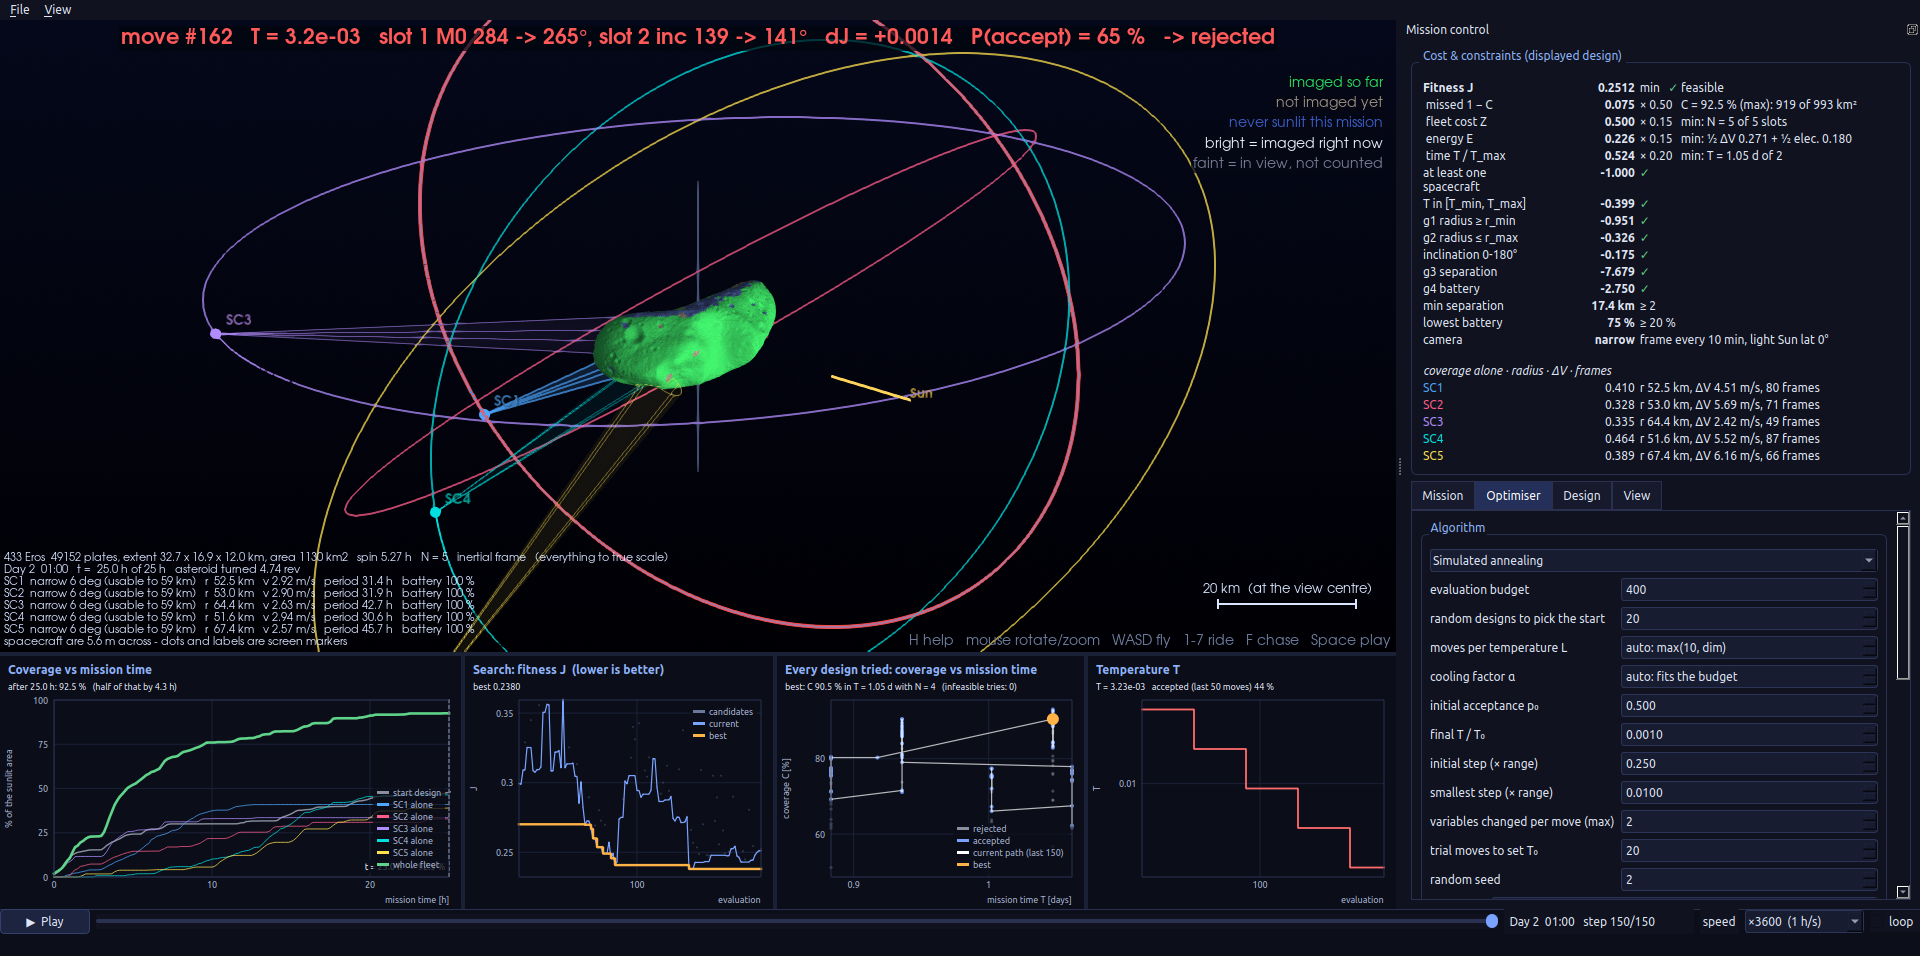
\includegraphics[width=\textwidth]{Figures/gui_sa.png}
\caption{The viewer while \ac{SA} runs: 3D scene with the current fleet (left), objectives,
constraints and optimiser settings (right), live charts of coverage, fitness, designs tried and
temperature (bottom).}
\label{fig:gui}
\end{figure}
